% !TEX root = ../InterpolatingOTFR.tex

\section{Numerical results}
\label{sec-numerics}

This section presents a numerical implementation of the computation of geodesics for our metric. The source code to reproduce these results is available online\footnote{\url{https://github.com/lchizat/optimal-transport/}}.

\subsection{Discretization}

The numerical resolution of the dynamical optimal transport problem is often performed with first order methods using proximal splitting algorithms (\cite{benamou2000computational}, \cite{papadakis2014optimal}).  These methods extend with no difficulties to the case of transport with sources, as long as the proximal operator of the new functional can be easily computed. In order to compare a few models of optimal transport with source, we implemented a Douglas-Rachford proximal splitting algorithm on a staggered grid, in the footsteps of \cite{papadakis2014optimal}. The introduction of the source term comes with a few adjustments so we describe the numerical method that we implemented, in the case of a transport problem in 1-D for simplicity (but the scheme works in arbitrary dimension).

\paragraph{Centered and staggered grids.}

\begin{figure}
 \centering
  \resizebox{0.40\linewidth}{!}{
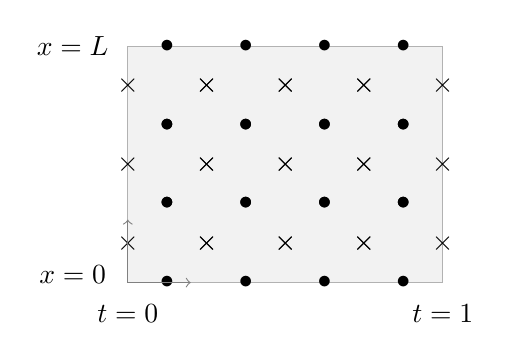
\begin{tikzpicture}
	\filldraw[color=black!30, fill=black!5] (-.5,-.5) rectangle (3.5,2.5);
	\foreach \x in {0,...,3}
   	 \foreach \y in {0,...,2} 
	 {
	\pgfmathparse{\x+0.5}\let\a\pgfmathresult
	\pgfmathparse{\y+0.5}\let\b\pgfmathresult
	\pgfmathparse{\x-0.5}\let\c\pgfmathresult
	\pgfmathparse{\y-0.5}\let\d\pgfmathresult
       	\draw[black,minimum size=5pt] (\x,\y) node {$\blacksquare$} ;
	\draw (\a,\y) node {$\times$} ; %[red!80]
	\draw  (\x,\b) node {$\bullet$} ; 
	\draw  (\c,\y) node {$\times$} ; 
	\draw  (\x,\d) node {$\bullet$} ; 
	}
	
	\draw[->, black!50] 	(-.5,-.5)    	-- 	(-.5,.3);
	%\draw       	(-1.4,1.) 	node {Space};
	\draw	(-1.2,-.4) node {$x=0$};
	\draw	(-1.2,2.5) node {$x=L$};
	
	\draw[->,black!50] 	(-.5,-.5) 	-- 	(.3,-.5);
	%\draw       	(1.5,-.9) 	node {Time};
	\draw 	(-.5,-.9)  	node {$t=0$};
	\draw 	(3.5,-.9) 	node {$t=1$};
\end{tikzpicture}
        }
\caption{($\blacksquare$) centered and ($\times$, $\bullet$) staggered grids. The grey rectangle is the space-time domain and here $N=3$, $T=4$.}
\label{fig: grids}
\end{figure}

%\todo{Gab: why not taking $L=1$ ?}

We consider the space domain $[0,L]$ and the time domain $[0,1]$. We denote $N$ the number of dicretization points in space and $T$ the number of discretization points in time. The centered grid is an equidistant discretization of the interior of the space-time domain $[0,L] \times [0,1]$, namely
\[
\mathcal{G}_c = \left\{ \left( x_i=L\frac{i-1/2}{N}, t_j=\frac{j-1/2}{T} \right): 1 \leq i \leq N, \, 1 \leq j \leq T \right\}
\]
and the variable discretized on the centered grid are denoted
\[
V = (\rho,\M,\Z) \in \mathcal{E}_c = (\R^{\mathcal{G}_c })^3.
\]
Remark that the boundaries are not included in the centered grid. There are as many staggered grids as there are dimensions, defined as
\[
\mathcal{G}_s^x = \left\{ (x_i = L\frac{i-1}{N}, t_j=\frac{j-1/2}{T}) :  1\leq i\leq N+1, \, 1\leq j \leq T \right\}\, ,
\]
\[
\mathcal{G}_s^t = \left\{ (x_i = L\frac{i-1/2}{N}, t_j=\frac{j-1}{T}) :  1\leq i\leq N, \, 1\leq j \leq T+1 \right\}\, , 
\]
and the variables discretized on the staggered grid are denoted by
\[
U = (\bar{\rho},\bar{\M},\bar{\Z}) \in \mathcal{E}_s = \R^{\mathcal{G}_s^t }\times \R^{\mathcal{G}_s^x }\times \R^{\mathcal{G}_c } .
\]
The source $\Z$ is discretized on the centered grid because there is no differentiation operator acting on this variable in the definition of the continuity constraint. Figure \ref{fig: grids} gives an illustration of the centered and staggered grids.

%%
\paragraph{Discrete continuity constraint.}
The discrete continuity constraint with boundary conditions is defined as the set
\begin{equation}
\label{eq_discretecontinuity}
\mathcal{CE} = \left\{   U= (\bar{\rho},\bar{\M},\bar{\Z}) \in \mathcal{E}_s :  AU = f_0 ,\, A = \left[
\begin{array}{c} 
\div - s_z \\ \hline 
s_b
\end{array}
\right]  , \, f_0 = \left[
\begin{array}{c}  
0  \\ \hline 
b_0
\end{array}
\right]  \right\}
\end{equation}
where $s_z : U \mapsto \bar{\zeta}$, $s_b$ selects the values of $U$ on the boundaries of the staggered grids and $b_0$  is a vector containing $\rho_0$, $\rho_1$ and zeros for the Neumann boundary conditions. The divergence operator $\div$ only acts on the components $(\bar{\rho},\bar{\M})$ of $U$, takes its values on the centered grid and is defined for $U\in \mathcal{E}_s$ as 
\[
\div(U)_{i,j} = \frac{N}{L} (\bar{\M}_{i+1,j}-\bar{\M}_{i,j}) + T (\bar{\rho}_{i,j+1}-\bar{\rho}_{i,j}) \, .
\]

%%%%%%%%%%%%%%%%%%%%%%
%%%%%%%%%%%%%%%%%%%%%%
\paragraph{Discrete functional.}

First, we use \thref{rescaling} and bring ourselves back to the case $\kappa = 1$ by a space rescaling: this allows to obtain a simpler proximal operator. The discrete functional is defined, for $V \in \mathcal{E}_c$, as $\ifoncN(V) \defeq \sum_{k\in\mathcal{G}_c } f(\rho_k,\M_k,\Z_k)$ with 
\[
f(\rho_k,\M_k,\Z_k) \defeq \frac{|\M_k|^2 + \Z_k}{2\rho_k} \, .
\]

%%%%%%%%%%%%%%%%%%%%
\paragraph{Interpolation operator.}
Since the continuity constraint and the functional $\ifoncN$ are not defined on the same grid, we need to keep two variables $(U,V)\in \mathcal{E}_s \times \mathcal{E}_c$ and to add an interpolation constraint between them, i.e.\ we require $V=\mathcal{I}(U)$ where $I$ is the midpoint interpolation operator 
\[
I(U)_{i,j} = \left( \frac{\bar{r}_{i,j+1}+\bar{r}_{i,j}}{2},\frac{\bar{m}_{i+1,j}+\bar{m}_{i,j}}{2},\bar{z}_{i,j} \right) \, .
\]

%%%%%%%%%%%%%%%%%%%%

\paragraph{Discrete optimization problem}
The discrete convex optimization problem that we aim to solve as an approximation of the continuous problem \eqref{dual} reads then
\begin{equation*}
\min_{U,V} \,  \ifoncN(V) + \iota_{\mathcal{CE}}(U) + \iota_{\{V=\mathcal{I}(U)\}} (U,V) \, .
\end{equation*}

%%%%%%%%%%%%%%%%%%%%%%
\subsection{Minimization algorithm}

\paragraph{Proximal methods and the Douglas Rachford algorithm.}

A popular class of first order methods for solving non-smooth convex optimization problems, so-called proximal splitting schemes, replaces the explicit gradient descent step by an implicit descent step using the so-called proximal operator. For a proper, convex, l.s.c.\ function $F$ defined on a Hilbert space $\mathcal{H}$ with values in $\R\cup +\infty$, the proximal operator is the single-valued map defined as
\[
	\prox_{\gamma F}(x) = \argmin_{\bar{x}\in \mathcal{H}} \frac12 \Vert x - \bar{x}  \Vert^2 + \gamma F(\bar{x}) \, .
\]
If $F$ is smooth, the optimality condition imply that $\bar{x} \defeq \prox_{\gamma F}(x)$ should satisfy $\bar{x} = x-\gamma \nabla F(\bar{x})$, justifying the common interpretation of the proximal operator as an implicit gradient step. 
%For the indicator function of a convex set, the proximal operator is the projection on this set.
A minimizer of $F$ can be found by successively applying the proximal operator, but for complicated functions without structure, computing the proximal operator can be as difficult as solving the whole minimization problem. 
However, if the function is the sum of simple terms, minimization can be performed by so-called \emph{proximal splitting} methods. 
%There are several ways to combine proximal operators in order to minimize the sum of functions. 
The one we implemented is the Douglas Rachford algorithm which allows to minimize the sum of two convex, proper, l.s.c.\ functions $G_1$ and $G_2$ with the following iterative scheme: choose two initial points $(z^{(0)},w^{(0)})\in \mathcal{H}^2$ and define the sequence
\begin{align*}
	w^{(l+1)} &= w^{(l)}+ \alpha (\prox_{\gamma G_1}(2z^{(l)}-w^{(l)})-z^{(l)}), \\
	z^{(l+1)} &= \prox_{\gamma G_2} (w^{(l+1)}) \, .
\end{align*}
If $0<\alpha<2$ and $\gamma >0$, one can show thant $z^{(l)} \rightarrow z^*$ a minimizer, see \cite{combettes2007douglas}. Depending on which functions we take as $G_1$ and $G_2$, we obtain various algorithms; in our code we used
\[
	G_1(U,V) = \iota_{\mathcal{CE}}(U) + \ifoncN(V) \quad \text{and} \quad G_2(U,V) = \iota_{V=\mathcal{I}(U)}(U,V) \, . 
\]
For a detailed review of proximal splitting algorithms, we refer the reader to \cite{combettes2011proximal}. Let us now compute the proximal operators.

%%%%%%%%%%%%%%%%%%%%%%%%%%%
\paragraph{Computing $\prox_{\gamma \ifoncN}$.}

The proximal operator of the functional $\ifoncN$ can be computed in closed form. The following result is a direct adaptation of \cite{papadakis2014optimal}.

\begin{proposition}
One has
\[
\forall \, V \in \mathcal{E}_c, \quad \prox_{\gamma \ifoncN}(V) = \left( \prox_{\gamma \foncN}(V_k)\right)_{k \in \mathcal{G}_c}
\]
where, for all $(\tilde{\rho},\tilde{\M}, \tilde{\Z}) \in \R \times \R^d \times \R$,
\[
\prox_{\gamma \foncN}(\tilde{\rho},\tilde{\M}, \tilde{\Z})  =
\begin{cases}
 \left( \rho^*, \frac{\rho^* \, \tilde{\M}}{\rho^* + \gamma},\frac{\rho^* \, \tilde{\Z}}{\rho^* + \gamma} \right) & \text{if $\rho^*>0$,}\\
 ( 0, 0, 0) & \text{otherwise},
\end{cases}
\]
and $\rho^*$ is the largest real root of the third order polynomial equation in $X$
\[
 P[X] = (X-\tilde{\rho})(X+\gamma)^2 - \frac{\gamma}{2} (|\tilde{\M}|^2+\tilde{\Z}^2) \, .
 \]
\end{proposition}

%%%%%%%%%%%%%%%%%%%%%%%%%%%
\paragraph{Computing $\proj_{\mathcal{CE}}$.}

The proximal operator of $\iota_{\mathcal{CE}}$ is the projection on the affine set $\mathcal{CE}$, which can be computed for $U \in \mathcal{E}_s$ as
 \begin{eqnarray}
\mathcal{P}_\mathcal{CE} (U) & = & U + A^* (A A^*)^{-1}(b_0 -AU) \\
& = & \mathcal{P}_B (U) - (Id-I_b)(s_z^* -\div^*) S^{-1} (s_z - \div ) (\mathcal{P}_B (U))
\end{eqnarray}
where $S=(\div - s_z)(Id - s_b^* s_b)(-\nabla - s_z^*)$ is the Schur complement of $AA^*$, $I_b$ is the identity on the boundaries on zero everywhere else and $\mathcal{P}_B$ is the projection on the boundary constraints. Given $p$, we can find $u$ satisfying $Su=p$ by solving $\Delta u -u + p=0$ on the centered grid with Neumann boundary conditions (on the staggered grids). In the Fourier domain, this equation reads
\[
\left[ 1 + (2- 2\cos( \pi m /N) )N/L + (2- 2\cos( \pi n/T) )T \right]   \hat{u}[m,n] = \hat{p}[m,n] \, .
%\left( 5 -2 \cos (2i\pi m/N) -2 \cos (2i\pi n/T) \right) \hat{u}[m,n] = h^2 \hat{p}[m,n] \, . %less general
\]
The DCT-II transform (with inverse DCT-III ) which coefficients are given by
\[
\hat{u}[k] = \sum_{n=1}^{N} u[n] \cos \left[ \frac{\pi}{N} (n+\frac{1}{2})k  \right]
\]
is adapted to our boundary conditions.

%%%%%%%%%%%%%%%%%%%%%%%%%%%%
\paragraph{Compute $\proj_{V = \mathcal{I}(U)}$.}
The projection is given for all couples $(U_0,V_0) \in (\mathcal{E}_s, \mathcal{E}_c )$ by 
\[
\proj_{V = \mathcal{I}(U)} (U_0,V_0) = (U^*, \mathcal{I}(U^*))
\]
with $U^*=Q^{-1}(U_0+\mathcal{I}^*V_0)$ and $Q=Id+\mathcal{I}^*\mathcal{I}$.
As $Q$ is a tridiagonal matrix, LU factorization techniques allow to efficiently invert the system.
%%%%%%%%%%%%%%%%%%%%%%%%%%%%
%\paragraph{Other proximal operators.}
%[???]


%%%%%%%%%%%%%%%%%%%%%%%%%
%%%%%%%%%%%%%%%%%%%%%%%%%
\subsection{Experiments}
%%%%%%%%

\begin{figure}[hbt]
 \centering
%
\begin{subfigure}{0.5\linewidth} 
\centering
 \resizebox{1.\linewidth}{!}{
\includegraphics{images/gaussian_p2q0}
}
\caption{Standard transport $W_2$}
\label{subW2}
\end{subfigure}%
%
\begin{subfigure}{0.5\linewidth} 
\centering
  \resizebox{1.\linewidth}{!}{
\includegraphics{images/gaussian_p2L2}
}
\caption{$L^2$ penalization on the source}
\label{subL2}
\end{subfigure}%

\begin{subfigure}{0.5\linewidth} 
\centering
 \resizebox{1.\linewidth}{!}{
\includegraphics{images/gaussian_p2q1}
}
\caption{Partial transport with $c_l=0.3$}
\label{subPT1}
\end{subfigure}%
%
\begin{subfigure}{0.5\linewidth} 
\centering
 \resizebox{1.\linewidth}{!}{
\includegraphics{images/gaussian_p2q1_small}
}
\caption{Partial transport with $c_l = 0.15$}
\label{subPT2}
\end{subfigure}

\begin{subfigure}{0.5\linewidth} 
\centering
  \resizebox{1.\linewidth}{!}{
\includegraphics{images/gaussian_p2q2}
}
\caption{$\WF_{\kappa}$ with $c_l =0.3$}
\label{subWF1}
\end{subfigure}%
%
\begin{subfigure}{0.5\linewidth} 
\centering
  \resizebox{1.\linewidth}{!}{
\includegraphics{images/gaussian_p2q2_small}
}
\caption{$\WF_{\kappa}$ with $c_l = 0.15$}
\label{subWF2}
\end{subfigure}
\caption{Comparison of interpolations for densities on the segment $[0,1]$:  $\rho_0$ (gray),  $\rho_1$ (blue),  $\rho_{t=1/2}$  (red), $\omega_{t=1/2}$ (black),  $\zeta_{t=1/2}$ (yellow). We indicate by $c_l$ the theoretical maximum distance a Dirac can travel, which is a function of $\kappa$.}
\label{fig:gaussians}
\end{figure}

%%%
\paragraph{Transport of Gaussian bumps.}

Let us first explore a synthetic case where the initial and final measures have the same mass. This case is shown on Figure \ref{fig:gaussians}. 
The initial and the final measures are both composed of two Gaussian densities of mass $1$ and $2$ supported on the segment $\Om=[0,1]$. The modes of the bumps are located at, from left to right, $0.2$, $0.3$, $0.65$ and $0.9$. The problem is discretized with $N=256$ samples in space and $T=11$ samples in time. The peculiar location of the Gaussian bumps allows to highlight the variations of the behavior of the geodesics, which is highly dependent on the metric and on the parameter $\kappa$. 
%
For the $W_2$ geodesic (Figure \ref{subW2}), the rightmost grey bump is split in half and a part of it travels to the left side of the graph, giving a interpolated measure which, for some applications, is not so natural. The effect of a non-homogeneous functional is visible on Figure \ref{subL2}, where we penalized the $L^2$ norm of the source $\Z$ in the functional. Non-homogeneity makes the density matter: in this case, the source is spread because low densities are favored. 
%
Consider now the partial transport geodesics: on Figure \ref{subPT1}, we fixed the maximum distance mass can travel to $2\kappa=0.3$, while on Figure \ref{subPT2}, that distance is $2\kappa=0.15$. We observe, as expected, that the domain $\Om=[0,1]$ is split in an active and an inactive set. Also note that as the $TV$ cost is not strictly convex, geodesics are not unique and what happens in the inactive set depends on the initialization of the algorithm.
%
Finally, Figures \ref{subWF1} and \ref{subWF2} display the geodesics at $t=1/2$ for the $\WF_{\kappa}$ metric with the \emph{cut locus} distances set, respectively, at $\pi \kappa=0.3$ and $\pi \kappa = 0.15$. Note that there is a slight similarity between the configuration here and the hypotheses of \thref{pairsdiracs}, and the observed behavior can be expected if we extrapolate the conclusions of that Theorem. In the first case, we obtain a geodesic consisting of two travelling bumps which inflate or deflate. While in the second configuration, only one bump travels as $\pi \kappa$ is now smaller than the distance between the two bumps at the right. 

%%%%%%%%%%%%%%%%%%%
% SYNTHETIC
%%%%%%%%%%%%%%%
\paragraph{Synthetic 2D experiments.}
We now turn our attention to a synthetic example on the domain $\Om=[0,1]^2$. The initial density $\rho_0$ is the indicator of the ring of center $(\frac12, \frac12)$, internal diameter $0.5$ and external diameter $0.7$. The final density $\rho_1$ is the pushforward of $\rho_1$ by a random smooth map and thus $\rho_0(\Om)=\rho_1(\Om)$. The domain is discretized on a centered grid of $64\times 64$ samples in space and $T=12$ samples in time. We compare on Figure \ref{fig: synthetic rho} the geodesics for four different metrics: $d_{FR}$, $W_2$, partial optimal transport (with $2\kappa=0.2$) and $\WF_{\kappa}$ (with $\kappa \pi = 0.4$). Notice that the two first rows thus show the limit geodesics for $\WF_{\kappa}$ when $\kappa$ tends to $0$ or $+\infty$ (see \thref{limitmodels}).

Figure \ref{fig: synthetic details} helps to better understand the geodesics. On the top row, the velocity field shows that the $W_2$ geodesic transports a lot of mass to the bottom left protuberance. On the contrary, metrics allowing local variations of mass (partial transport and $\WF_{\kappa}$), attenuate the component of the velocity field which is tangential to the ring, behavior which is more consistent with the intuitive solution. Finally, by looking at the source maps in the bottom row, we see the inactive sets of partial optimal transport with well defined edges and how this behavior strongly differs to that of $\WF_{\kappa}$ geodesics.

Figure \ref{fig: synthetic rho distance} displays another experiment intended to illustrates how the geodesics behave when a lot of transport is involved. The measures $\rho_0$ and $\rho_1$ have same total mass, the domain $\Om=[0,1]^2$ is discretized on a centered grid with $44 \times 44$ samples in space and $T=12$ samples in time. We show the geodesics for $W_2$, partial optimal transport (with $2\kappa=0.5$) and $\WF_{\kappa}$ (with $\kappa \pi = 0.5$).


\begin{figure}
 \centering
  \resizebox{1.0\linewidth}{!}{
\begin{tikzpicture}
\filldraw[color=black!5, fill=black!5] (-1.5,-1.) rectangle (.5,1);
\filldraw[color=black!5, fill=black!5] (11.5,-1.) rectangle (13.5,1);
\node (1r1) at (-0.5,0) {\includegraphics{images/circle_p2q0_r1}};
% p0q2
\node (3r2) at (2,2.25) {\includegraphics{images/circle_p0q2_r3}};
\node (3r3) at (4,2.25) {\includegraphics{images/circle_p0q2_r5}};
\node (3r4) at (6,2.25) {\includegraphics{images/circle_p0q2_r7}};
\node (3r5) at (8,2.25) {\includegraphics{images/circle_p0q2_r9}};
\node (3r6) at (10,2.25) {\includegraphics{images/circle_p0q2_r11}};
% p2q0
\node (0r2) at (2,.75) {\includegraphics{images/circle_p2q0_r3}};
\node (0r3) at (4,.75) {\includegraphics{images/circle_p2q0_r5}};
\node (0r4) at (6,.75) {\includegraphics{images/circle_p2q0_r7}};
\node (0r5) at (8,.75) {\includegraphics{images/circle_p2q0_r9}};
\node (0r6) at (10,.75) {\includegraphics{images/circle_p2q0_r11}};
% p2q1
\node (1r2) at (2,-.75) {\includegraphics{images/circle_p2q1_r3}};
\node (1r3) at (4,-.75) {\includegraphics{images/circle_p2q1_r5}};
\node (1r4) at (6,-.75) {\includegraphics{images/circle_p2q1_r7}};
\node (1r5) at (8,-.75) {\includegraphics{images/circle_p2q1_r9}};
\node (1r6) at (10,-.75) {\includegraphics{images/circle_p2q1_r11}};
%p2q2
\node (2r2) at (2,-2.25) {\includegraphics{images/circle_p2q2_r3}};
\node (2r3) at (4,-2.25) {\includegraphics{images/circle_p2q2_r5}};
\node (2r4) at (6,-2.25) {\includegraphics{images/circle_p2q2_r7}};
\node (2r5) at (8,-2.25) {\includegraphics{images/circle_p2q2_r9}};
\node (2r6) at (10,-2.25) {\includegraphics{images/circle_p2q2_r11}};

\node (1r7) at (12.5,0) {\includegraphics{images/circle_p2q0_r13}};

\draw[->] 	(1r1)    	-- 	(3r2);
\draw[->] 	(1r1)    	-- 	(0r2);
\draw[->]  	(1r1)    	-- 	(1r2);
\draw[->] 	(1r1)    	-- 	(2r2);
%\draw[dashed,color=black!30] (2,.9) --(10,0.9);
%\draw[dashed,color=black!30] (2,-1) -- (10,-1);
\draw[->]  	(3r6)    	-- 	(1r7);
\draw[->]  	(2r6)    	-- 	(1r7);
\draw[->] 	(0r6)    	-- 	(1r7);
\draw[->]  	(1r6)    	-- 	(1r7);
\draw[->]  	(-.5,-3)    	-- 	(12.5,-3);

\draw[dotted]        (2,0) -- (10,0);
\draw[dotted]        (2,-1.5) -- (10,-1.5);
\draw[dotted]        (2,1.5) -- (10,1.5);
\draw 	(-.5,-3.)  		node {$\bullet$};
\draw 	(-.5,-3.2)  		node {$t=0$};
\draw 	(12.5,-3.2)  	node {$t=1$};
\draw 	(6,-3.2)  	node {$t=0.5$};
\draw 	(-.5,-1.5)  	node {$\rho_0$};
\draw 	(12.5,-1.5)  	node {$\rho_1$};

\end{tikzpicture}
        }
\caption{Geodesics between $\rho_0$ and $\rho_1$ for four metrics:  Fisher-Rao (1st row),  $W_2$  (2nd row),  partial optimal transport (3rd row),  $\WF_{\kappa}$  (4th row).}
\label{fig: synthetic rho}
\end{figure}
%%%%%%%%%%%%%%%%%%%%%
%%%%%%%%%%%%%%%%%%%%%

\begin{figure}[ht]
 \centering
       
\begin{subfigure}{0.3\linewidth} 
\centering
 \resizebox{1.\linewidth}{!}{
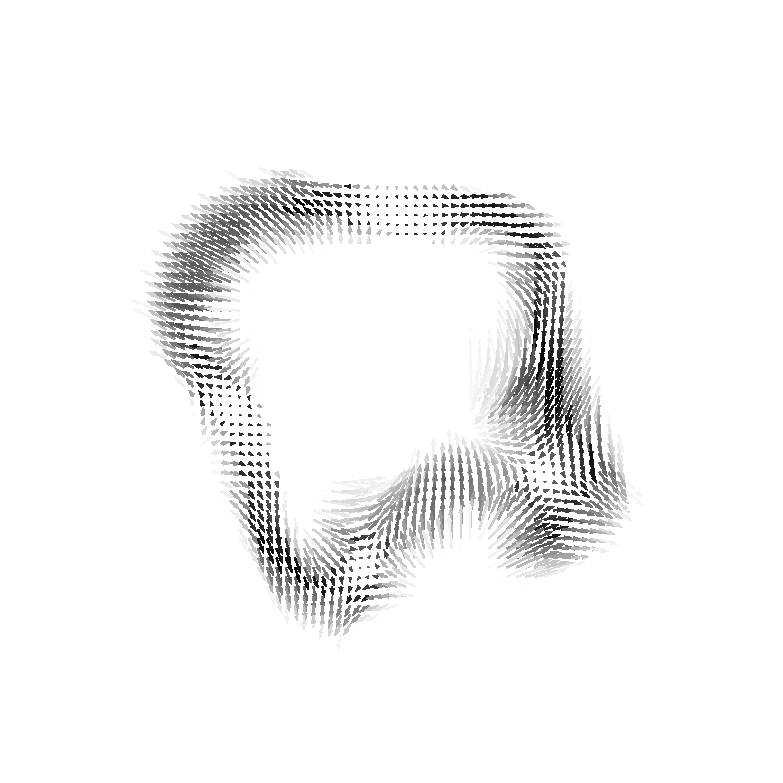
\includegraphics[clip,trim=2cm 2cm 2cm 2cm]{images/circle_p2q0_v}
}
\caption{$W_2$}
\end{subfigure}%
%
\begin{subfigure}{0.3\linewidth} 
\centering
 \resizebox{1.\linewidth}{!}{
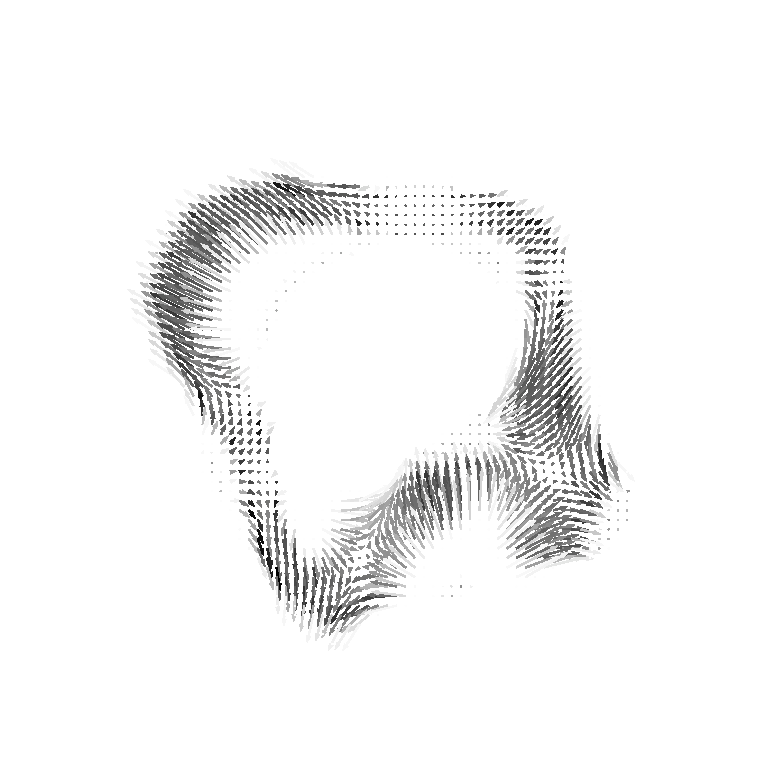
\includegraphics[clip,trim=2cm 2cm 2cm 2cm]{images/circle_p2q1_v}
}
\caption{Partial transport}
\end{subfigure}%
%
\begin{subfigure}{0.3\linewidth} 
\centering
  \resizebox{1.\linewidth}{!}{
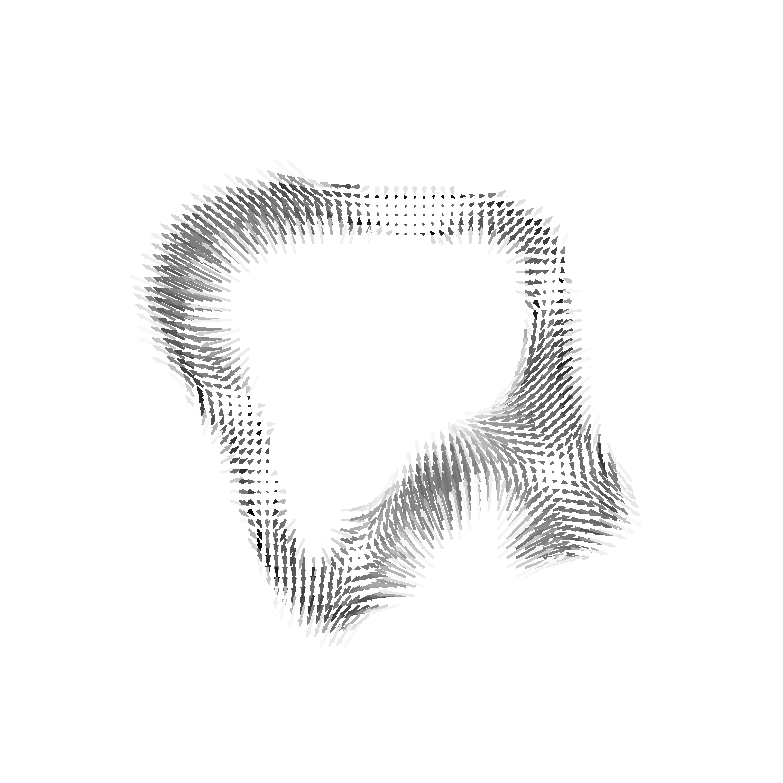
\includegraphics[clip,trim=2cm 2cm 2cm 2cm]{images/circle_p2q2_v}
}
\caption{$\WF_{\kappa}$}
\end{subfigure}

%
\begin{subfigure}{0.25\linewidth} 
\centering
 \resizebox{1.\linewidth}{!}{
\includegraphics[clip]{images/circle_p2q1_z6}
}
\caption{Partial transport}
\end{subfigure}%
%
\begin{subfigure}{0.25\linewidth} 
\centering
  \resizebox{1.\linewidth}{!}{
\includegraphics[clip]{images/circle_p2q2_z6}
}
\caption{$\WF_{\kappa}$}
\end{subfigure}

\caption{First row: velocity field $v = \omega/\rho$ at time $t=1/2$. The higher $\rho$, the darker the arrow. Second row: source $\zeta$ at time $t=1/2$. Blue stands for negative density and red for positive.}
\label{fig: synthetic details}
\end{figure}

\begin{figure}
 \centering
  \resizebox{1.0\linewidth}{!}{
\begin{tikzpicture}
\filldraw[color=black!5, fill=black!5] (-1.2,-1.45) rectangle (.2,-.05);
\filldraw[color=black!5, fill=black!5] (11.8,-1.45) rectangle (13.2,-.05);
\node (1r1) at (-0.5,-.75) {\includegraphics{images/linevar/linevar_p2q0_r1}};
% p2q0
\node (0r2) at (2,.75) {\includegraphics{images/linevar/linevar_p2q0_r3}};
\node (0r3) at (4,.75) {\includegraphics{images/linevar/linevar_p2q0_r5}};
\node (0r4) at (6,.75) {\includegraphics{images/linevar/linevar_p2q0_r7}};
\node (0r5) at (8,.75) {\includegraphics{images/linevar/linevar_p2q0_r9}};
\node (0r6) at (10,.75) {\includegraphics{images/linevar/linevar_p2q0_r11}};
% p2q1
\node (1r2) at (2,-.75) {\includegraphics{images/linevar/linevar_p2q1_r3}};
\node (1r3) at (4,-.75) {\includegraphics{images/linevar/linevar_p2q1_r5}};
\node (1r4) at (6,-.75) {\includegraphics{images/linevar/linevar_p2q1_r7}};
\node (1r5) at (8,-.75) {\includegraphics{images/linevar/linevar_p2q1_r9}};
\node (1r6) at (10,-.75) {\includegraphics{images/linevar/linevar_p2q1_r11}};
%p2q2
\node (2r2) at (2,-2.25) {\includegraphics{images/linevar/linevar_p2q2_r3}};
\node (2r3) at (4,-2.25) {\includegraphics{images/linevar/linevar_p2q2_r5}};
\node (2r4) at (6,-2.25) {\includegraphics{images/linevar/linevar_p2q2_r7}};
\node (2r5) at (8,-2.25) {\includegraphics{images/linevar/linevar_p2q2_r9}};
\node (2r6) at (10,-2.25) {\includegraphics{images/linevar/linevar_p2q2_r11}};

\node (1r7) at (12.5,-.75) {\includegraphics{images/linevar/linevar_p2q2_r13}};

%\draw[->] 	(1r1)    	-- 	(3r2);
\draw[->] 	(1r1)    	-- 	(0r2);
\draw[->]  	(1r1)    	-- 	(1r2);
\draw[->] 	(1r1)    	-- 	(2r2);
%\draw[dashed,color=black!30] (2,.9) --(10,0.9);
%\draw[dashed,color=black!30] (2,-1) -- (10,-1);
%\draw[->]  	(3r6)    	-- 	(1r7);
\draw[->]  	(2r6)    	-- 	(1r7);
\draw[->] 	(0r6)    	-- 	(1r7);
\draw[->]  	(1r6)    	-- 	(1r7);
\draw[->]  	(-.5,-3)    	-- 	(12.5,-3);

\draw[dotted]        (2,0) -- (10,0);
\draw[dotted]        (2,-1.5) -- (10,-1.5);
%\draw[dotted]        (2,1.5) -- (10,1.5);
\draw 	(-.5,-3.)  		node {$\bullet$};
\draw 	(-.5,-3.2)  		node {$t=0$};
\draw 	(12.5,-3.2)  	node {$t=1$};
\draw 	(6,-3.2)  	node {$t=0.5$};
\draw 	(-.5,-2.25)  	node {$\rho_0$};
\draw 	(12.5,-2.25)  	node {$\rho_1$};

\end{tikzpicture}
        }
\caption{Geodesics between $\rho_0$ and $\rho_1$ for three metrics: $W_2$ (1st row), partial optimal transport (2nd row),  $\WF_{\kappa}$ (3rd row). It is important to notice that $\rho_0$ is denser at the bottom left while $\rho_1$ is denser at the top right to better understand those geodesics.}
\label{fig: synthetic rho distance}
\end{figure}
%%%%%%%%%%%%%%%%%%%%%
%%%%%%%%%%%%%%%%%%%%%

%%%%%%%%%%%%%%%%%%%%%

%%%
\begin{figure}[ht]
 \centering
  \resizebox{1.0\linewidth}{!}{
\begin{tikzpicture}
\filldraw[color=black!5, fill=black!5] (-1.5,-1.25) rectangle (.5,1.25);
\filldraw[color=black!5, fill=black!5] (11.5,-1.25) rectangle (13.5,1.25);
\node (1r1) at (-0.5,0) {\includegraphics{images/brain_p2q2_r1}};

% p2q0
\node (0r2) at (2,1.25) {\includegraphics{images/brain_p2q2_r3}};
\node (0r3) at (4,1.25) {\includegraphics{images/brain_p2q2_r5}};
\node (0r4) at (6,1.25) {\includegraphics{images/brain_p2q2_r7}};
\node (0r5) at (8,1.25) {\includegraphics{images/brain_p2q2_r8}};
\node (0r6) at (10,1.25) {\includegraphics{images/brain_p2q2_r10}};
% p2q1
\node (1r2) at (2,-1.25) {\includegraphics{images/brain_p2q0_r3}};
\node (1r3) at (4,-1.25) {\includegraphics{images/brain_p2q0_r5}};
\node (1r4) at (6,-1.25) {\includegraphics{images/brain_p2q0_r7}};
\node (1r5) at (8,-1.25) {\includegraphics{images/brain_p2q0_r9}};
\node (1r6) at (10,-1.25) {\includegraphics{images/brain_p2q0_r11}};


\node (1r7) at (12.5,0) {\includegraphics{images/brain_p2q0_r13}};


\draw[->] 	(1r1)    	-- 	(0r2);
\draw[->]  	(1r1)    	-- 	(1r2);

\draw[dashed,color=black!30] (2,0) --(10,0.);
%\draw[dashed,color=black!30] (2,-1) -- (10,-1);


\draw[->] 	(0r6)    	-- 	(1r7);
\draw[->]  	(1r6)    	-- 	(1r7);
\draw[->]  	(-.5,-3)    	-- 	(12.5,-3);

%\draw[dotted]        (2,0) -- (10,0);
\draw 	(-.5,-3.)  		node {$\bullet$};
\draw 	(-.5,-3.2)  		node {$t=0$};
\draw 	(12.5,-3.2)  	node {$t=1$};
\draw 	(6,-3.2)  	node {$t=0.5$};
\draw 	(-.5,-1.5)  	node {$\rho_0$};
\draw 	(12.5,-1.5)  	node {$\rho_1$};

\end{tikzpicture}
        }
\caption{Geodesics between $\rho_0$ and $\rho_1$ for two metrics:   $W_2$ between rescaled densities (top row), $\WF_{\kappa}$ metric with $\pi\kappa=0.2$ (bottom row).}
\label{fig: brain interp}
\end{figure}

%
\begin{figure}
 \centering
       
\begin{subfigure}{0.3\linewidth} 
\centering
 \resizebox{1.\linewidth}{!}{
\includegraphics[clip,trim=2cm 1cm 2cm 1cm]{images/brain_p2q0_v_s3}
}
\caption{$v_{0.5}$ for $W_2$}
\label{fig: brain velo w2}
\end{subfigure}%
%
\begin{subfigure}{0.3\linewidth} 
\centering
 \resizebox{1.\linewidth}{!}{
\includegraphics[clip,trim=2cm 1cm 2cm 1cm]{images/brain_p2q2_v}
}
\caption{$v_{0.5}$ for $\WF_{\kappa}$}
\label{fig: brain velo wf}
\end{subfigure}%
%
\begin{subfigure}{0.33\linewidth} 
\centering
  \resizebox{1.\linewidth}{!}{
\includegraphics[clip,trim=0cm -0cm 0cm -0cm]{images/brain_p2q2_z}
}
\caption{$g_{0.5}$ for $\WF_{\kappa}$}
\label{fig: brain g wf}
\end{subfigure}

\caption{(a) and (b): velocity field $v=\omega/\rho$ for geodesics at time $t=1/2$. The higher $\rho_{0.5}$, the darker the arrow. (c) rate of growth $g=\Z/\rho$ at time $t=1/2$. Blue stand for negative density and red for positive and $g$ is set to zero when $\rho \approx 0$. Note that theoretically, (b) is the gradient field of (c).}
\label{fig: brain details}
\end{figure}

\paragraph{Biological images interpolation.}
Interpolating between shapes with varying masses is an important motivation for introducing this metric and is the object of our third and last numerical experiment. The initial and final densities $\rho_0, \rho_1$ are extracted form two segmented images of the same young brain taken at different times. This example is rather challenging for image matching algorithms: matter is creased, folded and grows unevenly. There are $89 \times 73$ samples in space, $12$ samples in time and the spatial domain is $\Om=[0,0.82]\times [0,1]$. We computed the geodesics for $W_2$ and for $\WF_{\kappa}$ with $\pi\kappa = 0.2$. We show on Figure \ref{fig: brain interp} the geodesics and on Figure \ref{fig: brain details} the velocity fields and the rate of growth a time $t=1/2$.

Most of the tissue growth is located at the bottom of the domain. Consequently, the velocity field associated to the $W_2$ geodesic is dominated by top to bottom components, as seen on Figure \ref{fig: brain velo w2}. To the contrary, the geodesic for the $\WF_{\kappa}$ metric manages to locally adapt the rate of growth, and the velocity field is far more consistent with the true evolution of the tissue. However, we retain some artifacts coming from optimal transport: some matter is teared off the brain lining and brought somewhere else to fill a need of mass. This behavior, inherent to the non-smooth nature of optimal transport plans, is clearly observed on Figure \ref{fig: brain interp} near the bulges that appear on the right and left sides of the brain.

Finally, let us recall the reader that, at optimality, the rate of growth $g$ is equal to the dual variable $\varphi$ and thus, the vector field on Figure \ref{fig: brain velo wf} is the gradient of the rate of growth on Figure \ref{fig: brain g wf}, which ranges in $[-0.05,0.18]$.



